\documentclass[a4paper,11pt]{article}

\usepackage{times}
%\setcounter{secnumdepth}{0} % sections are not getting numbered
\usepackage[english,serbian]{babel}


\usepackage[T1]{fontenc} 
%\usepackage[backend=biber,style=numeric,sortcites,sorting=nty,backref,natbib,hyperref]{biblatex} % bibliography

%\addbibresource{citation.bib} % file with references


\usepackage{comment}
\usepackage{amsfonts}
\usepackage{amsmath}
\usepackage{amsthm}
\usepackage{IEEEtrantools}
\usepackage{graphicx}
%\usepackage{cite}

%\usepackage{geometry}
%\usepackage{upgreek}
\usepackage[serbian]{babel}
%\usepackage{ulem}
%\usepackage{environ}
\usepackage{tikz}
\usepackage{color}
\usepackage{fancybox}

%\numberwithin{equation}{section}
\theoremstyle{definition} \newtheorem{deff}{Definicija}[section]
\theoremstyle{definition} \newtheorem{prim}[deff]{Primer}
\theoremstyle{plain} \newtheorem{teor}[deff]{Teorema}


\newcommand{\unija}[2]{#1 \cup #2}
\newcommand{\pres}[2]{#1 \cap #2}
\newcommand{\tnorm}{$t$-norm}
\newcommand{\tkonorm}{$t$-konorm}
\newcommand{\vect}[1]{\boldsymbol{\mathbf{#1}}}

\renewenvironment{proof}[1][\proofname]{{\bfseries #1.}}

\frenchspacing


\usepackage[a4paper,top=3cm,bottom=2cm,left=2cm,right=2cm,marginparwidth=1.75cm]{geometry}
%% Useful packages
\usepackage{mathrsfs}
\newsavebox\foobox
\newlength{\foodim}
\newcommand{\slantbox}[2][0]{\mbox{%
		\sbox{\foobox}{#2}%
		\foodim=#1\wd\foobox
		\hskip \wd\foobox
		\hskip -0.5\foodim
		\pdfsave
		\pdfsetmatrix{1 0 #1 1}%
		\llap{\usebox{\foobox}}%
		\pdfrestore
		\hskip 0.5\foodim
}}
\def\Laplace{\slantbox[-.45]{$\mathscr{L}$}}

%\usepackage[colorinlistoftodos]{todonotes}

\usepackage{caption}
\usepackage{subcaption}
\usepackage{changepage}
\usepackage{multirow}

\usepackage{blindtext}

\usepackage{tabularx}
\usepackage[export]{adjustbox}

\usepackage[utf8]{inputenc}
\usepackage[T1]{fontenc}
\usepackage{lmodern}
\usepackage{graphicx}
\usepackage{color}
\usepackage{listings}
\usepackage{amsmath}

%\usepackage[usenames,dvipsnames]{xcolor}
%\usepackage[colorlinks=true,linkcolor=blue]{hyperref}

\usepackage{amsfonts}
\usepackage{epstopdf}

\usepackage{float}

\usepackage[shortlabels]{enumitem}
\usepackage[yyyymmdd]{datetime}


\renewcommand{\figurename}{Slika}

\DeclareMathOperator*{\argmax}{\arg\max}
\graphicspath{{./images/}}

\usepackage{booktabs}

\usepackage{siunitx}

\usepackage{scalerel}






\sloppy

\epstopdfsetup{update} % only regenerate pdf files when eps file is newer

%%%%%%%% DOCUMENT %%%%%%%%
\setlength {\marginparwidth }{2cm}
\begin{document}
	
	%%%% Title Page
	\begin{titlepage}
		
		\newcommand{\HRule}{\rule{\linewidth}{0.5mm}} 							% horizontal line and its thickness
		\center 
		
		% University
		\textsc{\LARGE Elektrotehnički fakultet u Beogradu}\\[1cm]
		
		% Document info
		\textsc{\Large Distribuirani i frakcioni sistemi upravljanja}\\[0.2cm]
		\textsc{\large 13M051DIF}\\[1cm] 										
		\HRule \\[0.8cm]
		{ \huge \bfseries Projektovanje kontrolera primenom analiti"ckih i optimizacionih tehnika }\\[0.7cm]								% Assignment
		%\HRule \\[2cm]
		
		
		\large
		\vfill 
		\emph{Studenti:}\\
		Nikita Jokić 3279/2023\\[0.1cm]
		\emph{Mentor:}\\
		prof. dr Tomislav "Sekara\\[0.1cm]									
		{\large 2024}\\[2cm]
	\end{titlepage}
	\tableofcontents
	\newpage
	
	\section{Modeliranje sistema i projektovanje kontrolera}\label{sec:mod i an}
	\subsection{Uvod} 
	
	
	
	\newpage
	
	\subsection{Modeliranje sistema}\label{sec:modeliranje}
	
	Modeli su ključni elementi u projektovanju kontrolera jer omogućavaju simulaciju sistema i testiranje kontrolera u preliminarnoj fazi, u offline režimu. U slučaju korišćenja nelinearnih MPC kontrolera, zahteva se da model bude ugradjen u sistem.  \\
	
	U zavisnosti od pristupa koji se koristi, za dizajn kontrolera potrebni su različiti tipovi modela. Pristupi koji se primenjuju za podizanje klatna iz donjeg u gornji položaj, kao što su ad hoc i optimalno upravljanje zahtevaju nelinearne modele, jer sistem prati putanju u prostoru stanja koja prolazi kroz različite regione sa različitom dinamikom. S druge strane, održavanje klatna u gornjem položaju zahteva samo kontroler koji može raditi u nekoj okolini gornjeg položaja, te je za postizanje ovog cilja potreban samo linearni model.  \\
	
	Linearni modeli su mogu dobiti na dva načina: Jakobijan linearnizacijom nelinearnog modela u okolini želeljenog ravnotežnog stanja ili tehnikama identifikacije, gde se parametri linearnog modela procenjuju iz eksperimenata. U otvorenoj sprezi, gornji položaj je nestabilan, i ako se primeni mala smetnja na ulazu, izlazni signal će rasti bez ograničenja. Da bi se izbegao ovaj problem, potrebno je prikupiti podatke u slučaju kada se na sistem primeni upravljanje sa stabilnim kontrolerom.  Oblast identifikacije je detaljno proučavana krajem 1960-ih i početkom 1970-ih  \cite{identifikacija}. Glavni izazov je bio kako ukloniti šum koji se kontaminira sa ulazom i izlazom sistema.  \\
	
	
	
	\clearpage
	
	\subsubsection{Matlab model}\label{sec:matlab_model}
	
	Matlab model sistema je realizovan na osnovu izvedenih jedna"cina stanja. Prilikom implementcije modela inicijalno nije vo\dj eno ra"cuna o adekvatnoj diskretizaciji kontinualnog modela. Primenjena je Ojlerova aproksimacija $\dot{\mathbf{x}} \approx \frac{\mathbf{x}_{k+1} - \mathbf{x}_{k}}{\Delta t}$, $\mathbf{x}_{k}$ predstavlja k-ti odbirak kontinualnog stanja $\mathbf{x}$.
	
	\begin{equation} \label{eq:Ojler}
		\vect{x_{k+1}} = \vect{x_{k}} + \Delta t \vect{f}(\vect{x_k}, \vect{u_k}).
	\end{equation}.
	
	Me\dj utim, primena Ojlerove metode nije adekvatna za ovaj sistem usled velikih numeri"ckih gre"saka i nestabilnosti rezultuju\'ceg modela. Dodatnim korakom diskretizacije $\Delta t$ je mogu\'ce stabilizovati Ojlerovu metodu, ali to nije usvojeno kao prihvatljivo re"senje.\\
	
	
	
	\begin{figure}[!htb]
		\centering
		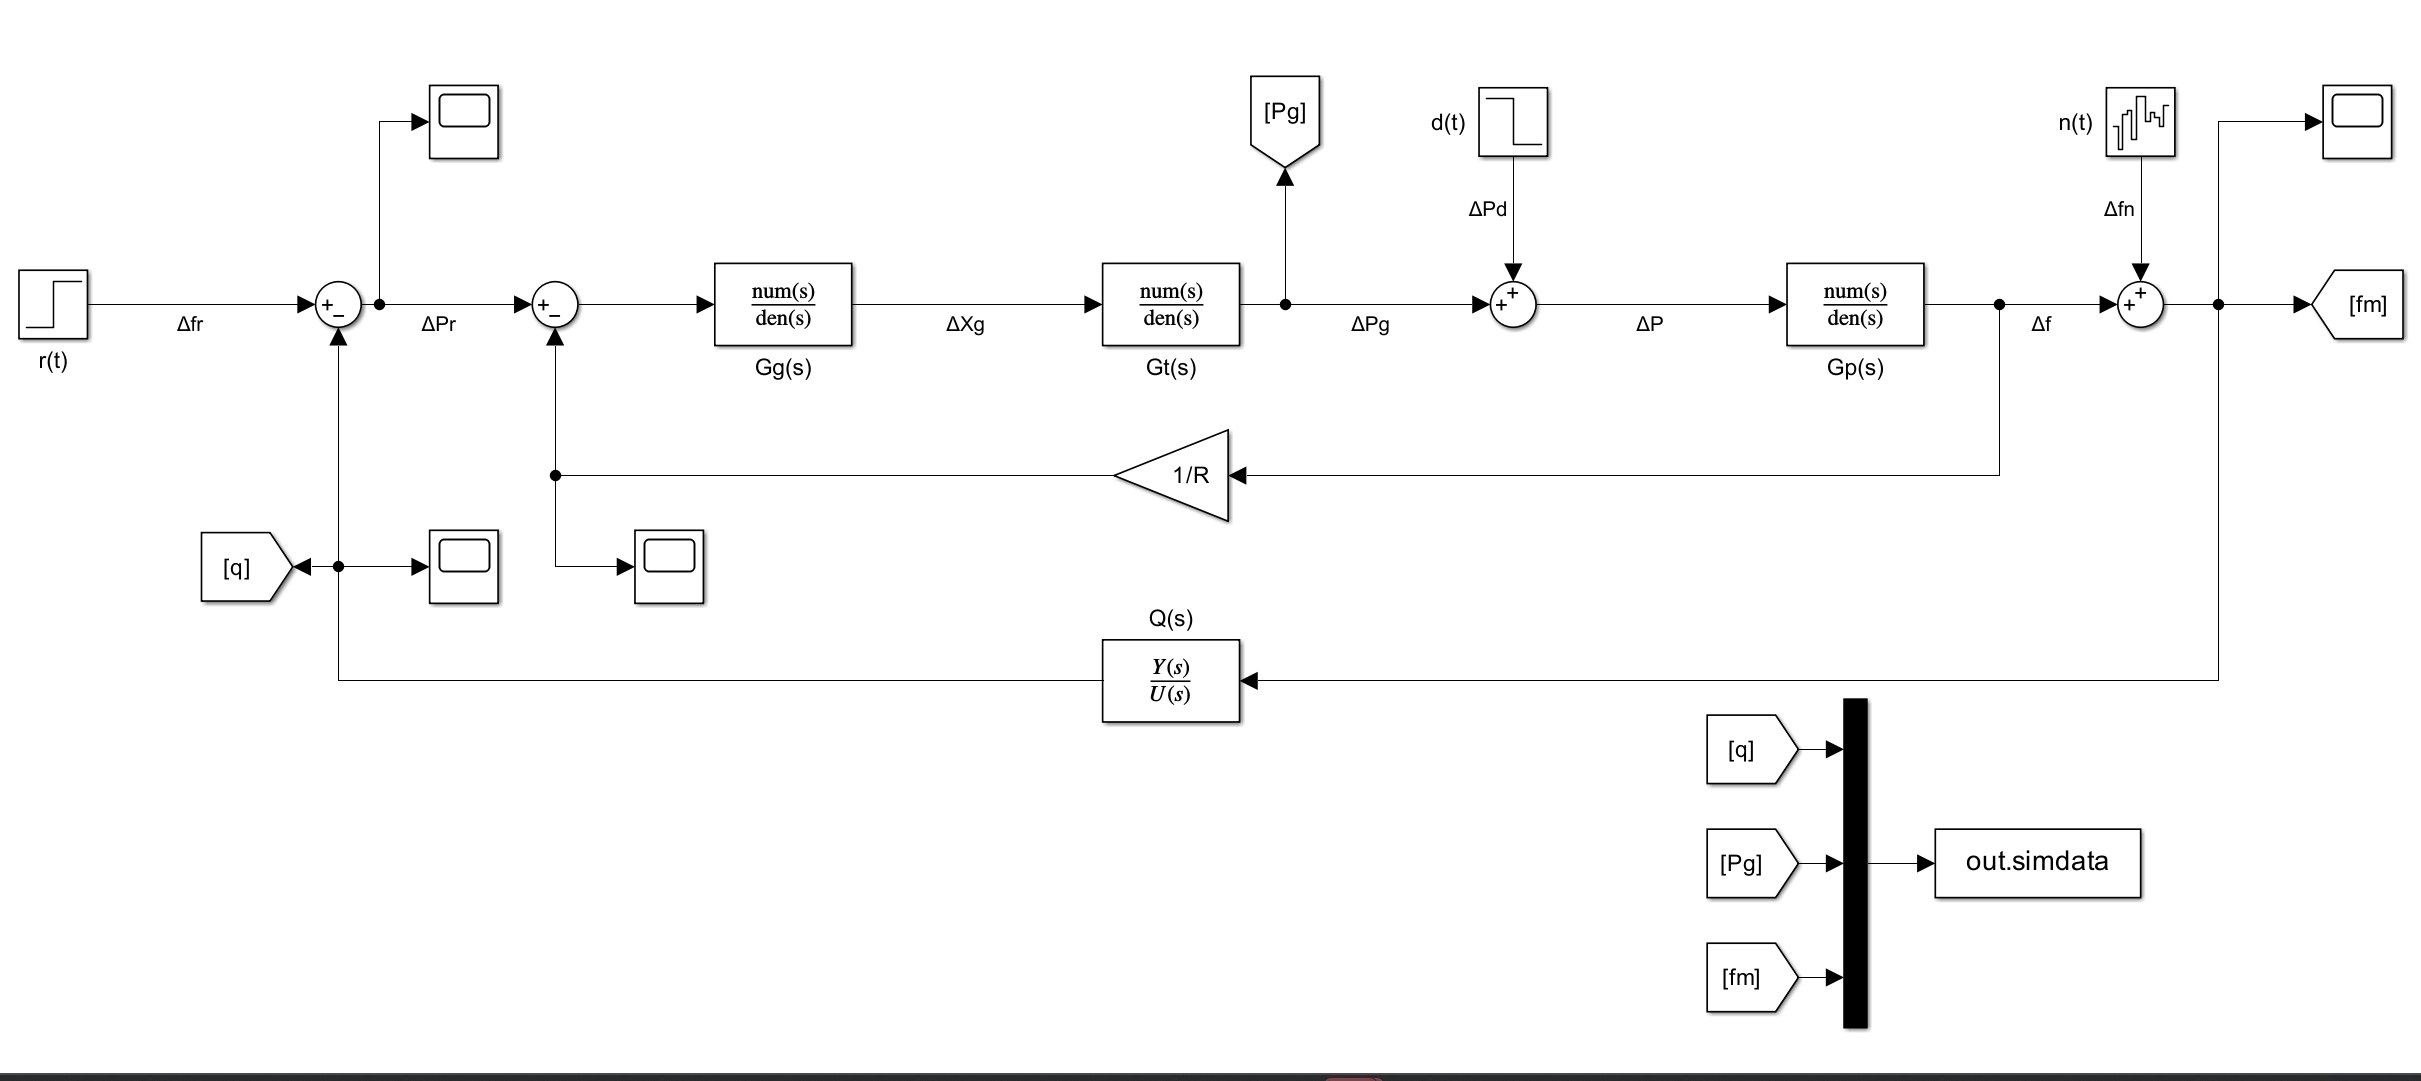
\includegraphics[width=0.45\linewidth]{slike/model.png}
		\caption{}
		\label{fig:model}
		
		\caption{Matlab model}
	\end{figure}
	
	
	
	
	
	
	\clearpage
	

	
	
	%\clearpage 
	\subsection{Analiti"cko projektovanje}
	\label{sec:linearizacija}
	

	
	\subsubsection{Optimizacija u vremenskom domenu} \label{sec:kontrolabilnost}
	

	
	
	\subsubsection{Optimizacija u frekvencijskom domenu}
	
	

	
	\subsection{Poremećaji u sistemu}
	
	U radu \cite{inicijalna} autor razmatra samo jedan izvor poreme\'caja i to step promenu stanja $\beta$. Razlog se ne navodi, ali je jasno da od 5 stanja datog sistema na stabilnost najve\'ci uticaj ima stanje $\beta$. U sekciji (\textbf{\ref{sec:kontrolabilnost}}) se razmatra uticaj stanja $\beta$ na kontrolabilnost sa stanovni"stva fizike. \\
	

	
	

	
	
	\newpage
	
	
	\section{Komparativna analiza projektovanih kontrolera} \label{sec:comp}
	\subsection{Diskusija}
	
	U ovoj sekciji su predstavljeni rezultati simulacija pomo\'cu kojih su verifikovani isprojektovani algoritmi. Implementiran je globalni LQR kao i \emph{gain scheduling}. Primena razli"citih kontrolera za stabilizaciju nije rezultovala velikim razlikama u trajektorijama, zbog toga u sekciji (\ref{sec:grafici}) su prikazani samo grafici sa \emph{gain scheduling} kontrolerom za stabilizaciju. \\ 
	
	Sve trajektorije su generisane \emph{offline} primenom egzaktnog modela. Prilikom dovo\dj enja klatna u uspravan generisano upravljanje i trajektorija u prostoru stanja se koriste kao referenca. Robustnost na gre"ske u modeliranju je ispitana naknadnim uvo\dj enjem $5\sigma$ gre"saka u odnosu na vrednosti iz tabele \ref{tab:tab1}.\\
	
	Svi razmatrani algoritmi su uspe"sno doveli klatno u uspravan polo"zaj. U slu"caju primene globalnog LQR kontroler se uklju"cuje ako je ugao $|\beta| \leq 16^o$, dok je \emph{gain scheduling} uvek uklju"cen. Nakon "sto ugao $|\beta|$ dostigne granicu od $16^o$ referentna trajektorija se postavlja na nulu i stabilizacija klatna se u potpunosti prepu"sta kontroleru.\\
	
	Prilikom simulacije prisutan je merni "sum. Analiza uticaja mernog "suma je izostavljena zbog prirode LQR kontroler. U pitanju je kontroler sa "cistim proporcionalnim dejstvom i kao takav nema osobine potiskivanja "suma (za razliku od kontrolera sa integralnim dejstvom). Mogu\'ce je delimi"cno smanjiti osetljivost na "sum prilikom projektovanja uvo\dj enjem ve\'ce cene upravljanja.\\
	
	Kako bi uporedili algoritme za uspravljanje klatna uvedene su slede\'ce metrike:
	\begin{itemize}
		\item $t_{16^o}$ - trenutak kad ugao $|\beta|$ pre\dj e granicu od $16^o$.
		\item $t_s$ - vreme smirenja ugla $\beta$.
		\item $E_u$ - energija upravlja"ckog signala, koristi se L2 norma.
	\end{itemize}
	Rezultati simulacija su tabelarno prikazani u sekciji (\ref{sec:tab}).\\
	
	Radi testiranja rada kontrolera u prisustvu poreme\'caja simulirana je step promena ugla $\beta$ u iznosu $\pm10^o$. Poreme\'caj se uvodi tek nakon "sto klatno uspe"sno dostigne gornji polo"zaj. Zbog toga se u sekciji (\ref{sec:por}) prikazuje samo jedan grafik. Algoritam za uspravljanje nema uticaja na poreme\'caje nakon "sto se dosegne gornji polo"zaj, kao "sto ne postoji razlika me\dj u LQR i \emph{gain scheduling} kontrolerima u gornjem polo"zaju.\\
	
	Prilikom generisanja trajektorija kori"s\'cen je RK4 algoritam opisan u sekciji (\ref{sec:matlab_model}) bez dodatnog umanjenja koraka integracije. Me\dj utim, prilikom dinamike klatna korak integracije je smanjen 4 puta. Cilj ovog pove\'canja preciznosti je da se elimini"su gre"ske usled neadekvatnog koraka odabiranja. \\
	
	Analizom grafika iz sekcije (\ref{sec:grafici}) mogu se uo"citi slede\'ce sli"cnosti me\dj u generisanim upravljanjima:
	\begin{itemize}
		\item Upravljanje generisano primenom MPC kvalitativno ima oblik kao upravljanje generisano primenom \emph{energy shaping}
		\item Upravljanje generisano primenom \emph{energy control} kvalitativno ima oblik kao upravljanje generisano primenom \emph{exponentiation of the pendulum position}
	\end{itemize} 
	
	
	
	
	
	
	
	
	
	
	
	
	
	
	
	\clearpage
	\subsection{Rezultati simulacije} \label{sec:grafici}
	\begin{figure}[!h]
		\centering
		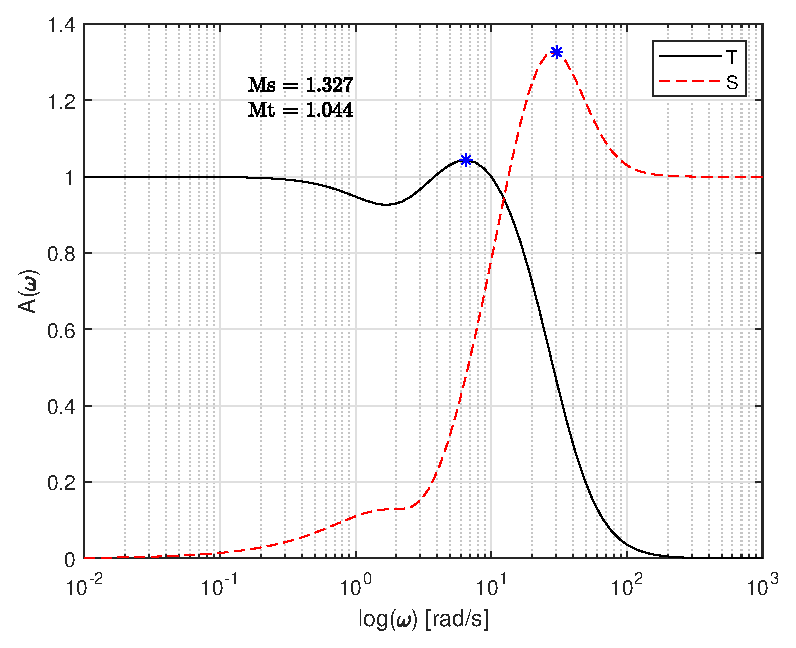
\includegraphics[width=0.47\linewidth]{slike/Ms_Mt_pidc.eps}
		\caption{Prikaz fukcije osetljivosti $S(\omega)$ i komplementarne osetljivosti $T(\omega)$ za PID$\text{c}_1$}
		\label{fig:MsMt_pidc}
	\end{figure}
	
	\begin{figure}[!h]
		\centering
		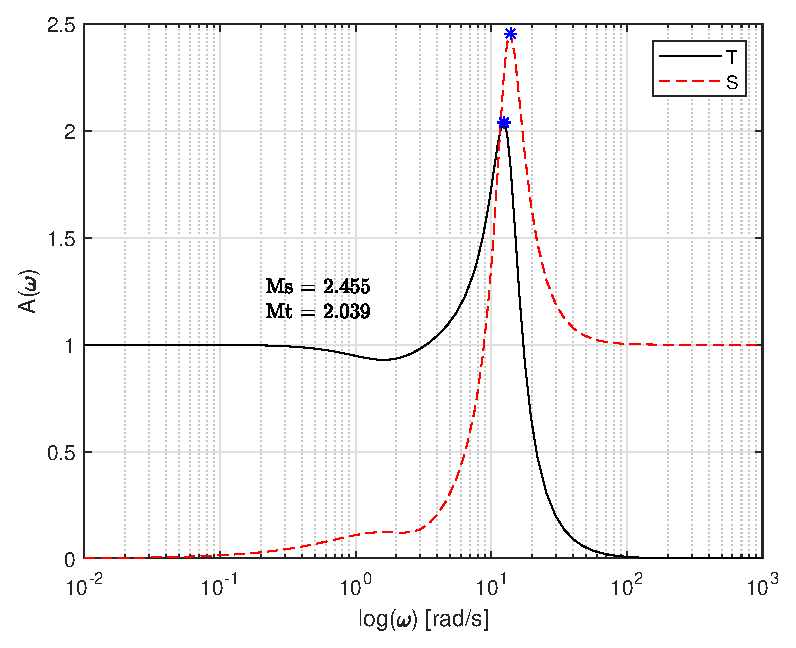
\includegraphics[width=0.47\linewidth]{slike/Ms_Mt_pid.eps}
		\caption{Prikaz fukcije osetljivosti $S(\omega)$ i komplementarne osetljivosti $T(\omega)$ za PID$_{\lambda=0}$}
		\label{fig:MsMt_pid}
	\end{figure}
	
	\begin{figure}[!h]
		\centering
		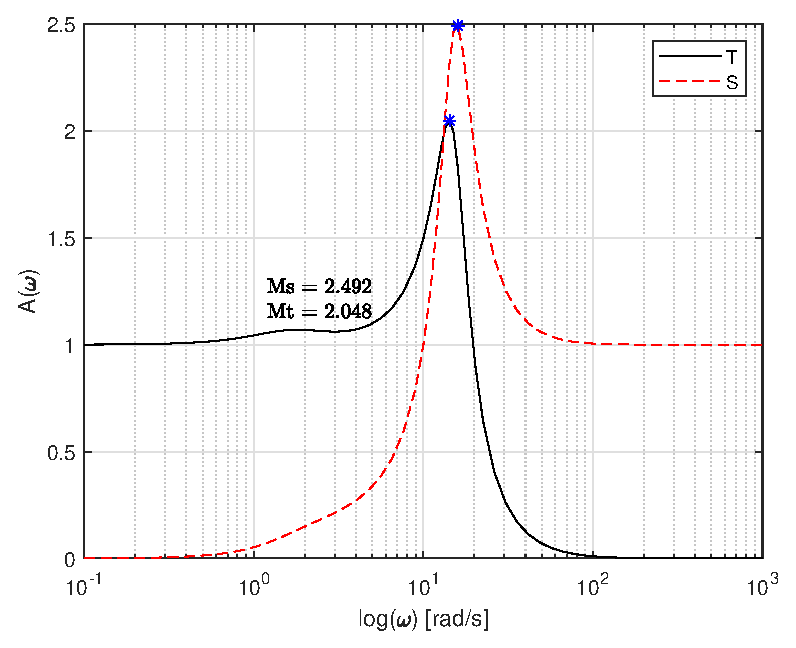
\includegraphics[width=0.47\linewidth]{slike/Ms_Mt_pid_lam.eps}
		\caption{Prikaz fukcije osetljivosti $S(\omega)$ i komplementarne osetljivosti $T(\omega)$ za PID$_{\lambda=0}$}
		\label{fig:MsMt_pid_lam}
	\end{figure}
	
	\begin{figure}[!h]
		\centering
		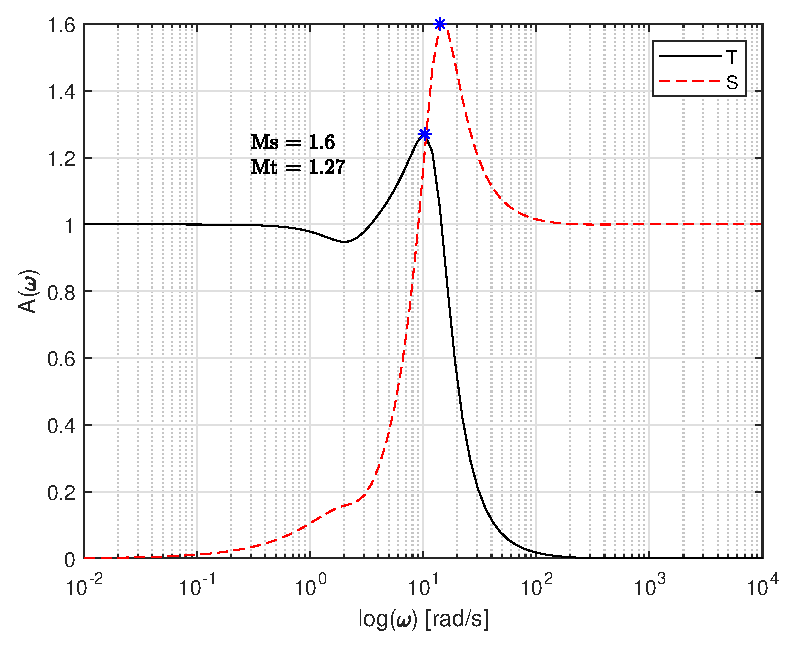
\includegraphics[width=0.6\linewidth]{slike/Ms_Mt_pid_opt.eps}
		\caption{Prikaz fukcije osetljivosti $S(\omega)$ i komplementarne osetljivosti $T(\omega)$ za PID$_{t}$}
		\label{fig:MsMt_pid_opt}
	\end{figure}
	
	\begin{figure}[!h]
		\centering
		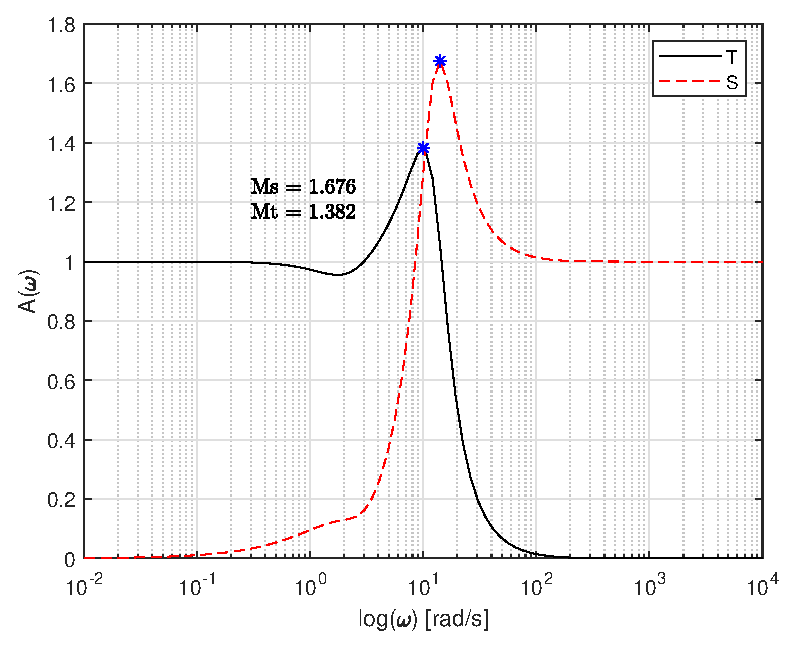
\includegraphics[width=0.6\linewidth]{slike/Ms_Mt_pid_optf.eps}
		\caption{Prikaz fukcije osetljivosti $S(\omega)$ i komplementarne osetljivosti $T(\omega)$ za PID$_{f}$}
		\label{fig:MsMt_pid_optf}
	\end{figure}
	\clearpage
	
	\begin{figure}[!h]
		\centering
		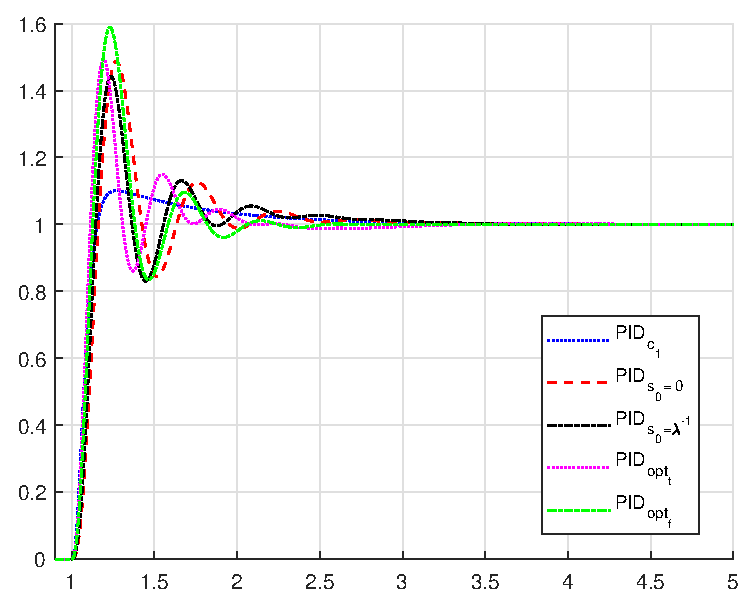
\includegraphics[width=0.6\linewidth]{slike/Pg_comparison_default.eps}
		\caption{Pore\dj{}enje odziva na promenu reference}
		\label{fig:Pg_default}
	\end{figure}
	
	\begin{figure}[!h]
		\centering
		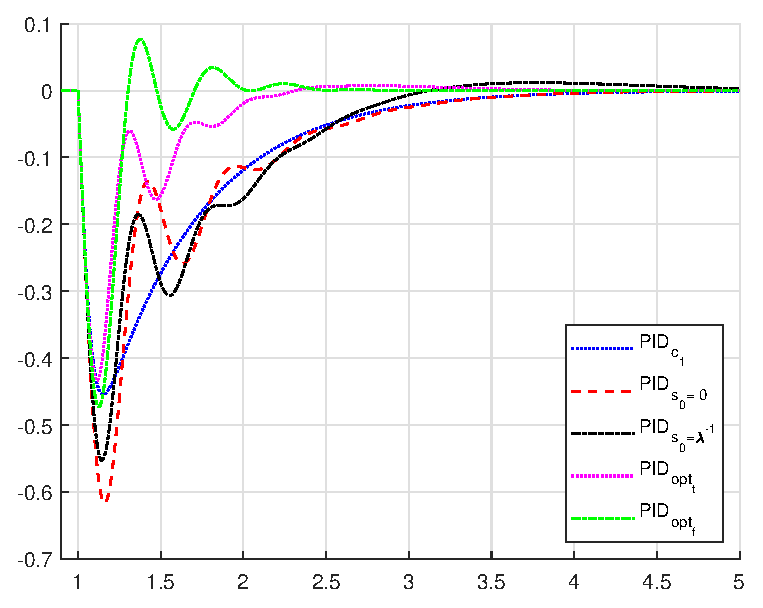
\includegraphics[width=0.6\linewidth]{slike/fm_comparison_default.eps}
		\caption{Pore\dj{}enje odziva na poreme\'caj}
		\label{fig:fm_default}
	\end{figure}
	
	\begin{figure}[!h]
		\centering
		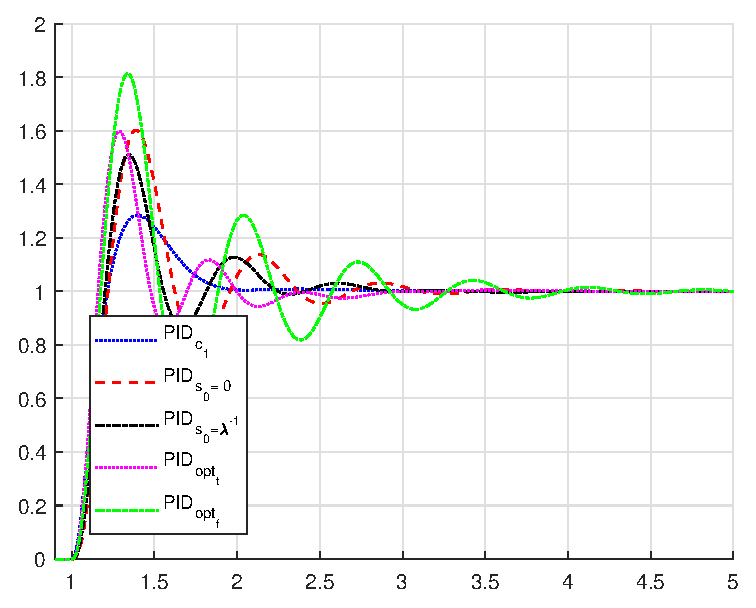
\includegraphics[width=0.6\linewidth]{slike/Pg_comparison_+50.eps}
		\caption{Pore\dj{}enje odziva na promenu reference, parametri uve\'cani za $50\%$}
		\label{fig:Pg_50}
	\end{figure}
	
	\begin{figure}[!h]
		\centering
		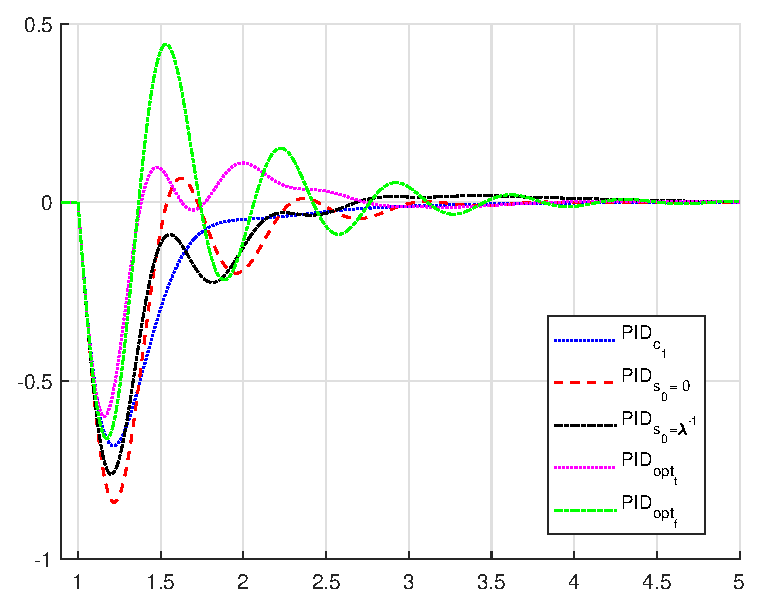
\includegraphics[width=0.6\linewidth]{slike/fm_comparison_+50.eps}
		\caption{Pore\dj{}enje odziva na poreme\'caj, parametri uve\'cani za $50\%$}
		\label{fig:fm_50}
	\end{figure}
	
\begin{figure}[!h]
	\centering
	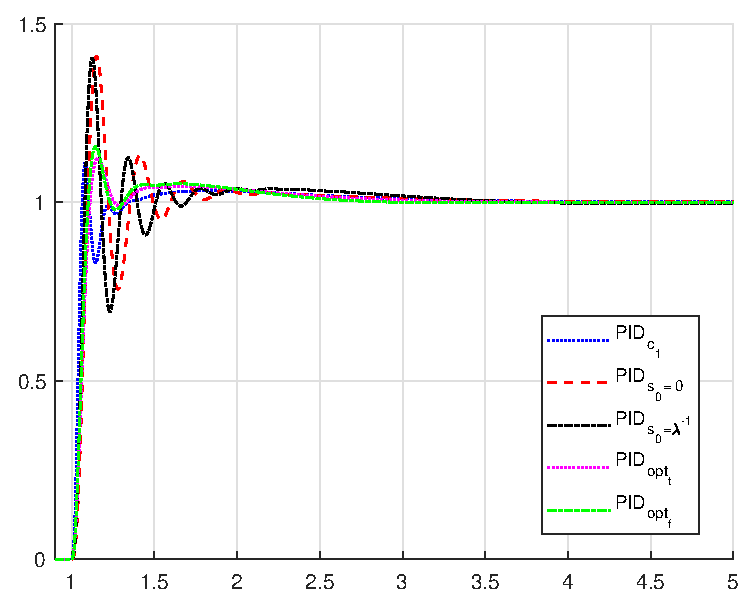
\includegraphics[width=0.6\linewidth]{slike/Pg_comparison_-50.eps}
	\caption{Pore\dj{}enje odziva na promenu reference, parametri smanjeni za $50\%$}
	\label{fig:Pg_-50}
\end{figure}

\begin{figure}[!h]
	\centering
	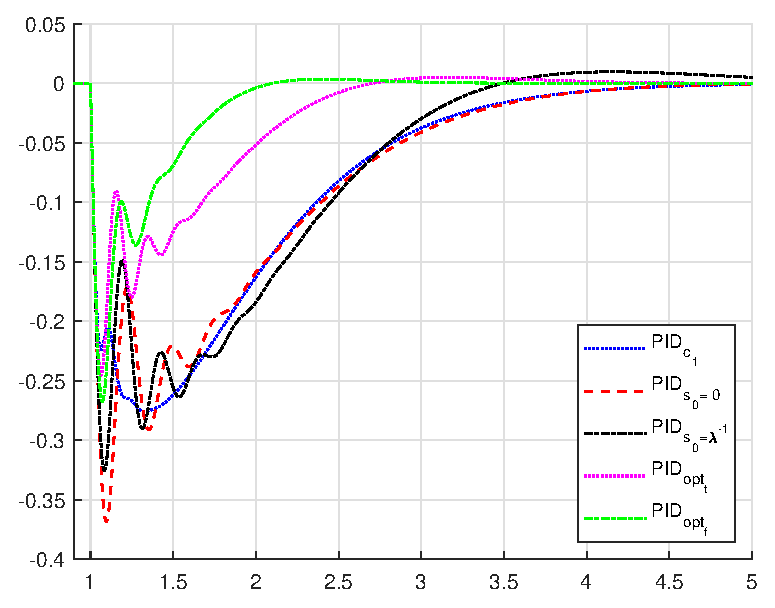
\includegraphics[width=0.6\linewidth]{slike/fm_comparison_-50.eps}
	\caption{Pore\dj{}enje odziva na poreme\'caj,
	parametri smanjeni za $50\%$}
	\label{fig:fm_-50}
\end{figure}

\begin{figure}[!h]
	\centering
	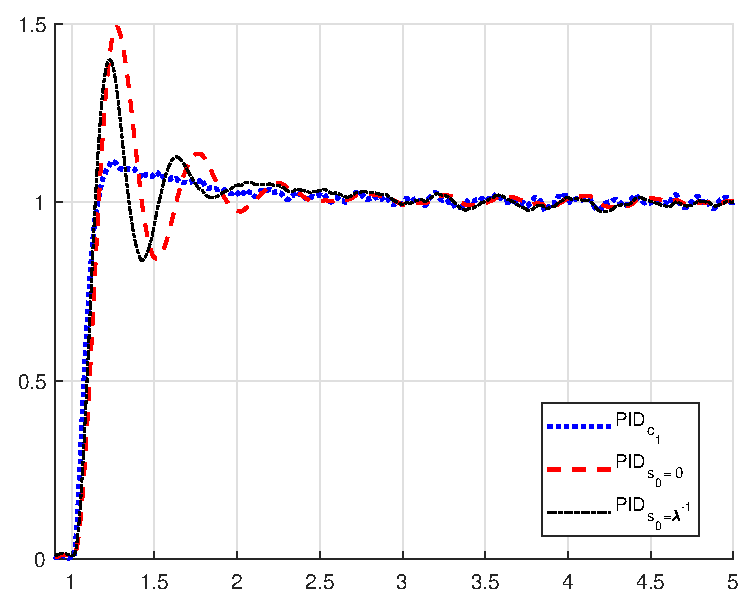
\includegraphics[width=0.6\linewidth]{slike/Pg_comparison_noise.eps}
	\caption{Pore\dj{}enje odziva na promenu reference u prisustvu "suma}
	\label{fig:Pg_noise}
\end{figure}

\begin{figure}[!h]
	\centering
	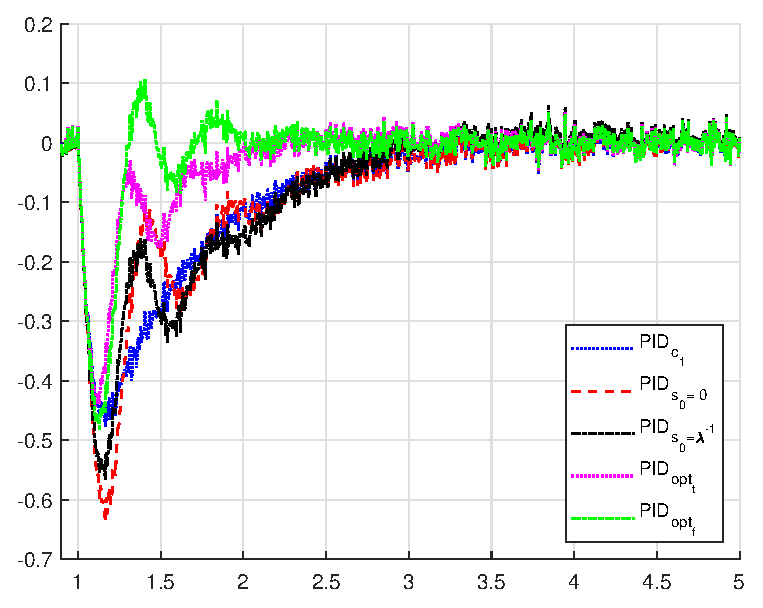
\includegraphics[width=0.6\linewidth]{slike/fm_comparison_noise.eps}
	\caption{Pore\dj{}enje odziva na poreme\'caj,
		u prisustvu "suma}
	\label{fig:fm_noise}
\end{figure}
	
	

	
	
	
	\clearpage
	\subsubsection{Tabelarni prikaz rezultata simulacije}\label{sec:tab}
	
	
	
		\begin{table}[!h]
			\resizebox{.75\textwidth}{!}{%
				\begin{tabular}{lllll}
					\hline
					\multicolumn{5}{c}{Pore\dj{}enje kontrolera, nominalni re"zim} \\ \hline
					& IAE      & IE        & ITAE      & TVd     \\ \hline
					PIDc                              & 67.9387  & -67.9387  & 112.8425  & \textbf{0.9080}  \\ \hline
					PID$_{s_0 = 0}$                   & 67.9410  & -67.9387  & 112.8597  & 1.4884  \\ \hline
					PID$_{s_0 = \frac{1}{\lambda}}$   & 70.0435  & -63.7952  & 120.1797  & 1.3725  \\ \hline
					PID$_t$                           & 29.6047  & -16.8988  & 46.8164   & 1.1080  \\ \hline
					PID$_f$                           & \textbf{22.4895}  & \textbf{-14.9049}  & \textbf{28.4012}   & 1.2957  \\ \hline
				\end{tabular}%
			}
			\label{tab:result_nominal}
		\end{table}
		
	\begin{table}[!h]
		\resizebox{.75\textwidth}{!}{%
			\begin{tabular}{lllll}
				\hline
				\multicolumn{5}{c}{Pore\dj{}enje kontrolera, parametri uve\'cani za $50\%$} \\ \hline
				& IAE      & IE        & ITAE      & TVd     \\ \hline
				PIDc                              & 67.9387  & -67.9387  & 99.8695  & \textbf{1.3648}  \\ \hline
				PID$_{s_0 = 0}$                   & 71.6303  & -67.9387  & 106.2790   & 2.3576  \\ \hline
				PID$_{s_0 = \frac{1}{\lambda}}$   & 73.2516  & -63.7947  & 116.3983   & 1.8473  \\ \hline
				PID$_t$                           & \textbf{43.0697}  & -16.8987  & \textbf{67.0920}   & 1.6956  \\ \hline
				PID$_f$                           & 77.1154  & \textbf{-14.9049}  & 131.8510   & 3.4103  \\ \hline
			\end{tabular}%
		}
		\label{tab:result_+50}
	\end{table}
	
		\begin{table}[!h]
		\resizebox{0.75\textwidth}{!}{%
			\begin{tabular}{lllll}
				\hline
				\multicolumn{5}{c}{Pore\dj{}enje kontrolera, parametri smanjeni za $50\%$} \\ \hline
				& IAE      & IE        & ITAE      & TVd     \\ \hline
				PIDc                              & 67.9387  & -67.9387  & 125.9439  & \textbf{0.5896}  \\ \hline
				PID$_{s_0 = 0}$                   &  67.9606  & -67.9387  & 126.0952   & 1.0112  \\ \hline
				PID$_{s_0 = \frac{1}{\lambda}}$   &  69.0071  & -63.7961  & 130.3229   & 1.0326  \\ \hline
				PID$_t$                           & 25.0244  & -16.8989  & 41.2495    & 0.7673  \\ \hline
				PID$_f$                           &  \textbf{16.0775}    & \textbf{-14.9049}  & \textbf{21.2812}   &0.6136  \\ \hline
			\end{tabular}%
		}
		\label{tab:result_-50}
	\end{table}
	
	\begin{table}[!h]
		\resizebox{0.75\textwidth}{!}{%
			\begin{tabular}{lllll}
				\hline
				\multicolumn{5}{c}{Pore\dj{}enje kontrolera u prisustvu "suma} \\ \hline
				& IAE      & IE        & ITAE      & TVd     \\ \hline
				PIDc                              & 81.9753  & -67.7478  & 209.9080  & \textbf{28.8642}  \\ \hline
				PID$_{s_0 = 0}$                   &  82.2774  & -67.6408  &  211.8215`   & 29.0482  \\ \hline
				PID$_{s_0 = \frac{1}{\lambda}}$   &  84.0861  & -63.5301  & 216.8843   & 28.9761  \\ \hline
				PID$_t$                           & 45.6514  & -16.7383   &  151.6361    &  28.9403
				  \\ \hline
				PID$_f$                           &  \textbf{41.2982}    & \textbf{-14.6598}  & \textbf{141.4925}   &29.0080
				 \\ \hline
			\end{tabular}%
		}
		\label{tab:result_noise}
	\end{table}
		
		
	


	
	\clearpage
	\section{Zaklju"cak}\label{sec:zakljucak}
	
	Na osnovu rezultata iz sekcije (\textbf{\ref{sec:tab}}) mo"ze se re\'ci da  izbor tipa kontrolera nije uvek o"cigledan. \emph{Gain scheduling} pristup rezultuje boljim performansama u slu"caju ve\'cih gre"saka u modelovanju, ali razlike u performansama su dovoljno male da mo"zda nije opravdano koristiti slo"zeniji kontroler. Primena 
	\emph{gain scheduling} zahteva projektovanje N puta vi"se kontrolera. Me\dj utim, i pored ve\'ce slo"zenosti ovaj prostup je jednostavniji za implementaciju od ve\'cine nelinearnih kontrolera i kao takav mo"ze predstavljati dobar kompromis izme\dj u slo"zenosti i performansi. "Sto se ti"ce strategija za uspravljanje klatna, pokazano je da upravljanje generisano primenom MPC tro"si ubedljivo najmanje energije. Ovaj rezultat je u skladu sa o"cekivanjima zbog oblika funkcije cene iz sekcije (\textbf{\ref{sec:OU}}). Ako se u obzir uzmu svi faktori kao dobar kompromis se name\'ce pristup na bazi \emph{energy shaping}, daleko je jednostavniji od MPC i rezultuje brzim odzivom uz prihvatljiv utro"sak energije.  \\
	
	Ovaj rad ima nekoliko nedostataka i ovde \'ce biti navedeni. Za razliku od autora rada \cite{inicijalna} ne vr"si se ispitivanje L1 norme. Kao "sto je re"ceno u sekciji (\textbf{\ref{sec:OU}}) razlog za to je problem sa konvergencijom. "Cak i u slu"cajevima kad algoritam konvergira rezultuju\'ce trajektorije su bile prakti"cno identi"cne. Zbog ovog manjka pouzdanosti je doneta odluka da se L1 norma u potpunosti elimini"se. Nije implementiran Kalmanov filtar zato "sto su u simulaciji sva stanja opservabilna. Me\dj utim, u radu autor navodi da je samo 3 od 5 stanja direktno merljivo, u toj situaciji je neophodno koristiti Kalmanov filtar. Mada primena klasi"cnog Kalmanovog nije u potpunosti opravdana zbog nelinearne prirode sistema. Za nelinearne sisteme ima vi"se smisla koristiti filtre kao "sto su pro"sireni Kalmanov filtar (eng. \emph{extended Kalman filter}) i neosetljivi Kalmanov filtar (eng. \emph{Unscented Kalman filter}). Pored navedenog jo"s jedan nedostatak je manjak detaljne analize robustnosti. Ispitivanje je sprovedeno tako "sto su svi parametri uve\'canji za $5\sigma$. Rigoroznije ispitivanje podrazumeva pretragu u prostoru parametara modela, kako bi prona"sli najgoru kombinaciju parametara. Ova pretraga se mo"ze znatno redukovati ukoliko se sprovede analiza simboli"cke funkcije prenosa linearizovanog sistema u gornjem polo"zaju. \\
	
	Prostor za budu\'ca istra"zivanja postoji. Mo"ze se sprovesti komparativna analiza brzine konvergencije i stabilnosti MPC u zavisnosti od tipa implementacije. U ovom radu je kori"s\'cena samo \emph{multiple shooting} metoda. O"cigledna nadogradnja na ovaj rad je primena MPC za stabilizaciju u gornjem polo"zaju uz primenu dovoljno brzog algoritma za rad u realnom vremenu. Ovaj pristup bi zahtevao kori"s\'cenje jo"s efikasnije biblioteke kao "sto je ACADOS \cite{acados}. ACADOS za razliku od CASADI stavlja manji akcenat na ta"cnost re"senja primenom br"zih solvera koji ne pronalaze nu"zno najbolje re"senje. Pored brzine prednost ACADOS-a je to "sto se implementirani kod lako spu"sta na mikrokontroler. U ovom radu su kori"s\'cene tipi"cne strategije u vidu nelinearnog upravljanja i MPC. Zanimljiva modifikacija ovog rada bi podrazumevala uzimanje u obzir malo egzoti"cnijih strategija kao "sto su u"cenje podsticanjem (eng. \emph{reinforced learning}) i primena genetskog algoritma (eng. \emph{genetic algorithm}) za optimizaciju upravljanja. 
	
	
	
	
	\newpage
	
	\begin{thebibliography}{9}
		\bibitem{inicijalna}
		\emph{Nonlinear control of an inverted pendulum}, António Samuel Ávila Balula, Thesis to obtain the Master of Science Degree in
		Engineering Physics 2016.
		
		\bibitem{energy_c}
		\emph{Swinging up the furuta pendulum and its stabi- ´
			lization via model predictive control.}, P. Seman, B. Rohal’-Ilkiv, M. Juhas, and M. Salaj.  Journal of Electrical Engineering, 64(3):152–158, 2013. ISSN
		13353632. doi: 10.2478/jee-2013-0022.
		\bibitem{ener_shaping}\emph{A normal form for energy shaping: application to the furuta pendulum}
		S. Nair and N. E. Leonard. 
		In Decision and Control, 2002, Proceedings of the 41st IEEE Conference on, volume 1, pages
		516–521. IEEE, 2002
		\bibitem{identifikacija}\emph{Identification of Dynamic System}, R. Isermann and M. Munchhof, Springer, 2011.
		
		\bibitem{mpc} \emph{https://en.wikipedia.org/wiki/Model\_predictive\_control}
		\bibitem{rk4}\emph{https://en.wikipedia.org/wiki/Runge\%E2\%80\%93Kutta\_methods}
		
		\bibitem{CASADI}\emph{https://web.casadi.org/}
		
		\bibitem{multiple_shooting}\emph{Nonlinear Model Predictive Control Using Multiple Shooting Combined with 
			Collocation on Finite Elements}, Jasem Tamimi and Pu Li.
		
		\bibitem{acados} \emph{https://github.com/acados/acados}
		
	\end{thebibliography}
\end{document}
